%!TEX TS-program = xelatex
%!TEX encoding = UTF-8 Unicode
%%========================================================
%%  编译方法(Windows, Mac OSX): 					
%%                    XeLaTeX 
%%                    biber
%%                    XeLaTeX
%%                    XeLaTeX
%%========================================================

%%%%%%%%%%%%%%%%%%%%%%%%%%%%%%%%%%%%%%%%%%%%%%%%%%%%%%%%%%
%            英文稿 文章模板:A4 纸, 五号字, 单列              
%%%%%%%%%%%%%%%%%%%%%%%%%%%%%%%%%%%%%%%%%%%%%%%%%%%%%%%%%%
\documentclass[English]{APSart}
%\usepackage{}  %添加自己论文需要的其他宏包

\ExecuteBibliographyOptions{gblocal = gb7714-2015, 
%							firstinits=true,
							gbpub = false,
							mincitenames = 1, % 要定义最后的分割符 (逗号, &, 和) , 前者:1 -> 一作等; 2-> 一作,二作 等
							maxcitenames = 2, % 2
							maxbibnames = 3,
							defernumbers=true
							}


\addbibresource{apsrefs-en.bib} % 加载bib文件(参考文献)

\begin{document}
%%
%%
%%%%%%%%%%%%%%%%%%%%%%%%%%%%%%%%%%%%%%%%%%%%%%%%%%%%%%%%%%%%%%%%
%%------------------ 编辑部提供的信息 ------------------------%%
%%%%%%%%%%%%%%%%%%%%%%%%%%%%%%%%%%%%%%%%%%%%%%%%%%%%%%%%%%%%%%%%
\newcommand{\pubvol}{XX}         % 卷号
\newcommand{\pubno}{X}           % 期号
\newcommand{\pubyear}{XXXX}      % 出版年份
\newcommand{\pubmonth}{XX}       % 出版月份
\newcommand{\enpubmonth}{XX}     % 出版月份
\newcommand{\ksym}{xx}           % 开始页码
\newcommand{\jsym}{xx}           % 结束页码
\newcommand{\receivedate}{Month Day, Year} % 论文收到日期
\newcommand{\modifydate}{Month Day, Year}  % 论文修改日期
\newcommand{\doino}{DOI:10.3969/j.issn.1001-4268.year.month.no}
\newcommand{\citationinfo}%
{citation information, provided by the APS Editorial when accepted}
%{LIU B W, ZHANG J, CHEN X P. \etitle\,[J]. Chinese J Appl Probab Statist, \pubyear, \pubvol(\pubno): \ksym--\jsym. }
%%

\apsnumber{APS-2024-001}             % 论文编号 --- 编辑部受理后产生

%%
%%%%%%%%%%%%%%%%%%%%%%%%%%%%%%%%%%%%%%%%%%%%%%%%%%%%%%%%%%%%%%%%
%%-------------------- 作者提供的信息 ------------------------%%
%%%%%%%%%%%%%%%%%%%%%%%%%%%%%%%%%%%%%%%%%%%%%%%%%%%%%%%%%%%%%%%%
\newcommand{\runenauthors}{Authors list}  
%Authors list:First Name (仅有一个作者时)
%            First Name, Second Name (仅有二个作者时)
%            First Name, et al. (超过两个作者时)
\newcommand{\cnfirstauthor}{一作姓名}
\newcommand{\cnsecondauthor}{二作姓名}
\newcommand{\cnfirstinst}{一作单位, 城市名, 邮政编码}
\newcommand{\cnsecondinst}{二作单位, 城市名, 邮政编码}
% 可添加更多作者及信息
\newcommand{\authorsinfo}{\textbf{作者信息}:~
	第一作者(出生时间--),~性别,~职称,~主要研究方向:~xxxxxx,~E-mail:xxxxx@xxxx.xxx.xx~;
	第二作者(出生时间--):~性别, 职称,主要研究方向:~xxxxxx,~E-mail:xxxxx@xxxx.xxx.xx~.}
\newcommand{\caemail}{abc@xyz.edu.cn}
\newcommand{\cntitle}{论文题目}
\newcommand{\cnkeywords}{关键词1, 关键词2, 关键词3, 关键词4.}
\newcommand{\cnclassno}{Oxxx.xx (网站: \url{http://www.ztflh.com/})}  % 中图分类号
\newcommand{\fundinfo}{This project was supported by Fund name (Grand No. 12345678).}
%% 中文摘要
\newcommand{\cnabstract}{摘要内容摘要内容摘要内容摘要内容摘要内容摘要内容摘要内容摘要内容摘要内容摘要内容摘要内容
	摘要内容摘要内容摘要内容摘要内容摘要内容摘要内容摘要内容摘要内容摘要内容摘要内容摘要内容摘要内容摘要内容.}
%%
%% 英文信息
\newcommand{\enfirstauthor}{First Name}
\newcommand{\ensecondauthor}{Second Name$^\star$}
\newcommand{\enfirstinst}{First Author's Working Unit, City, Zip Code, Country}
\newcommand{\ensecondinst}{Second Author's Working Unit, City, Zip Code, Country}
% 可添加更多作者及信息
\newcommand{\entitle}{English Title}
\newcommand{\enkeywords}{Keyword 1, Keyword 2, Keyword 3, Keyword 4.}
\newcommand{\amsno}{62xxx (Website:\url{https://mathscinet.ams.org/msc/})} % AMS Subject Claassification
%%
%% 英文摘要
\newcommand{\enabstract}{The abstract comes here! The abstract comes here! The abstract comes here! The abstract comes here!
	The abstract comes here! The abstract comes here! The abstract comes here! The abstract comes here! The abstract comes here!} %%
%%-------------------- 作者信息提供完毕 ------------------------%%
%% 论文标题页将自动生成
%% 作者转到后面的引言开始输入正文内容

%%%%%%%%%%%%%%%%%%%%%%%%%%%%%%%%%%%%%%%%%%%%%%%%%%%%%%%%%%%%%%%%
%        文章正文                                              %
%%%%%%%%%%%%%%%%%%%%%%%%%%%%%%%%%%%%%%%%%%%%%%%%%%%%%%%%%%%%%%%%

\title{\entitle %
\thanks{\zihao{-5}{~\fundinfo}}
}
\author{\textrm{\zihao{5} \enfirstauthor}\\[-2pt]
	(\zihao{-5} \enfirstinst) \\[1pt]
	\textrm{\zihao{5}\ensecondauthor}\\[-2pt]
	(\zihao{-5} \ensecondinst)
}
%%%%%%%%%%%%%%%%%%%%%%%%%%%%%%%%%%%%%%%%%%%%%%%%%%%%%%%%%%%%%%%%
% 作者姓名与单位 : 三种形式中选一种
% 后面中文摘要中的名字和单位参考中文模板的说明
% ---------------------
% 第一种形式: 仅有一个单位
% 作者列表
% (作者单位)
% ---------------------
% \author{\textrm{\zihao{5}\enfirstauthor}\\[-2pt]
% (\zihao{-5} \enfirstinst)
%}

% ---------------------
% 第二种形式: 二个单位 多个作者 --- 名字左右并列
% 作者列表1     作者列表2  
% (作者单位1)   (作者单位2)
% ---------------------
%\author{\textrm{\zihao{5}\enfirstauthor}\\[-2pt]
%     (\zihao{-5}\enfirstinst)
%     \and 
%     \textrm{\zihao{5} \ensecondauthor}\\[-2pt]
%     (\zihao{-5} \ensecondinst)
%}

% ---------------------
% 第三种形式: 不同单位 多个作者 -- 名字与单位上下并列
% \author{\textrm{\zihao{5} \cnfirstauthor}\\[-2pt]
%     (\zihao{-5} \cnfirstinst)\\[1pt]
%     \textrm{\zihao{5} \cnsecondauthor}\\[-2pt]
%     (\zihao{-5}\cnfirstinst)
%}
%
% 其他可视为上述三种的组合
% ---------------------
%%%%%%%%%%%%%%%%%%%%%%%%%%%%%%%%%%%%%%%%%%%%%%%%%%%%%%%%%%%%%%%

\date{}  % 这一行用来去掉默认的日期显示
\maketitle
\vspace{-6mm}
%%%%%%%%%%%%%%%%%%%%%%%%%%%%%%%%%%%%%%%%%%%%%%%%%%%%%%%%%%%%%%%%
%  英文文摘要
%%%%%%%%%%%%%%%%%%%%%%%%%%%%%%%%%%%%%%%%%%%%%%%%%%%%%%%%%%%%%%%%
\begin{center}
	\begin{minipage}[c]{14cm}
		\zihao{-5}
		\textbf{Abstract:}\quad\enabstract\\
		\textbf{Keywords:}\quad\enkeywords\\
		\textbf{2020 Mathematics Subject Classification:}\quad\amsno\\
		\rule[3mm]{14cm}{0.2pt}\vskip-4mm
		\textbf{Citation:}\quad \fullcite{Current2024}.
		\\  %\citationinfo
		\rule[3mm]{14cm}{0.2pt}
	\end{minipage}
\end{center}
\footnote[0]{\hskip-1.5mm
	$^\star$Corresponding author, E-mail: \caemail.}
\footnote[0]{Received on \receivedate{}. Revised on \modifydate{}.}\vspace{-1em}


%%%%%%%%%%%%%%%%%%%%%%%%%%%%%%%%%%%%%%%%%%%%%%%%%%%%%%%%%%%%%%%%
%  正文由此开始
%%%%%%%%%%%%%%%%%%%%%%%%%%%%%%%%%%%%%%%%%%%%%%%%%%%%%%%%%%%%%%%%
\baselineskip17.5pt
\pagewiselinenumbers   % 行号供审稿时用,投稿前可注释

%%%%%%%%%%%%%%%%%%%%%%%%%%%%%%%%%%%%%%%%%%%%%%%%%%%%%%%%%%%%%%%%
\section{Inroduction}
%%%%%%%%%%%%%%%%%%%%%%%%%%%%%%%%%%%%%%%%%%%%%%%%%%%%%%%%%%%%%%%%
This a \LaTeX{} English article template specially designed for Chinese Journal of Applied Probability and Statistics. 
%%%%%%%%%%%%%%%%%%%%%%%%%%%%%%%%%%%% %%%%%%%%%%%%%%%%%%%%%%%%%%%%
\section{Common Environments in \LaTeX{}}
%%%%%%%%%%%%%%%%%%%%%%%%%%%%%%%%%%%%%%%%%%%%%%%%%%%%%%%%%%%%%%%%

\subsection{Section Title}
We recommend tha authors only use thr first two levels of sections, i.e., \texttt{section} and \texttt{subsection}. Either ordered list with \texttt{enumerate} environment and non-ordered bullets with \texttt{itemize} environment are recommended for higher levels of sections. 
\begin{remark}
First letters in the section titles should be capitalized for this journal.  
\end{remark}
\subsection{Label Specification and Refer to}
For detailed description, see the template in Chinese version.
Here are some examples of lists, formulae, tables, figures, bibiliography, and their citations for your reference.

\subsubsection{Lists}
\begin{enumerate}[leftmargin=7.8mm,itemsep=-0.1ex,label=\arabic*)]
	\item item 1
	\item item 2
	\begin{enumerate}[leftmargin=7.8mm,itemsep=-0.1ex,label=(\alph*)]
		\item item 3
		\item item 4
	\end{enumerate}
\end{enumerate}

\begin{enumerate}[leftmargin=7.8mm,itemsep=-0.1ex,label=(\Roman*)]
	\item item 5
	\item item 6
\end{enumerate}

\subsubsection{Formulas}
Equations as a whole:
\begin{equation} \label{eq:1}
	\begin{aligned}
		Y & = \beta_0 + \beta_1 X + \varepsilon, \\
		\varepsilon & \sim N(0, \sigma^2). 
	\end{aligned}
\end{equation}

Equations independently or long equation with breaks:
\begin{align}
	\pi &= 3.1415926\cdots \nonumber \\
		&\approx  3.14.  \label{align-a1}
\end{align}

\subsubsection{Tables}
\begin{table}[htbp]
	\centering\zihao{-5}
	\caption{Table with booktabs and \texttt{multicolumn} command. Table with booktabs and \texttt{multicolumn} command. }\label{table:1}
	\vskip -5pt
	\begin{tabular}{cccccc}
		\toprule
		& \multicolumn{4}{c}{Scores} & \\
		\cmidrule(lr){2-5}
		Name & Calculus & Linear Algebra & Politics & Englsih & Total \\
		\midrule
		Alice & 90 & 85 & 92 & 88 & 355 \\
		Bob & 88 & 90 & 85 & 89 & 352 \\
		Carol & 92 & 87 & 88 & 93 & 360 \\
		\bottomrule
	\end{tabular}
\end{table}

\begin{table}[htbp]
	\centering\zihao{-5}
	\caption{Table with booktabs and \texttt{multirow} command.} 
	\vskip -5pt
	\begin{tabular}{ccc}
		\toprule
		Column 1 & Column 2 & Column 3\\ 
		\midrule
		\multirow{2}{*}{Multirow}&X&\multirow{2}{*}{Multirow}\\
		&X&\\
		X&\multirow{2}{*}{Multirow}&\multirow{2}{*}{Multirow}\\
		X&&\\
		\bottomrule
	\end{tabular}
\end{table}

\subsubsection{Figures}
\begin{figure}[htbp]
\centering
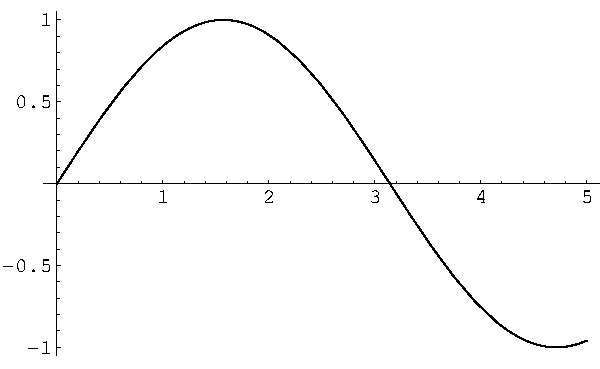
\includegraphics[width=0.6\textwidth]{figs/sin}
\vskip -5pt
\caption{A floating figure\label{fig:fig4}}
\end{figure}


\begin{example}
	One figure in one line, which is commonly used. See, for example, Figure \ref{fig:fig4}. 		
\end{example}

\begin{example}
	Two figures side by side, which are relatively independent with continuous numbers. See, for example, Figure \ref{mini:suba} and Figure \ref{mini:subb}. 		
\end{example}

\begin{example}
	Two sub figures side by side sharing the common figure number counter. Figure \ref{mini:subfigs} is created with command \verb/\subcaptionbox/ from \TeX{} package \texttt{subcaption}.  	
\end{example}

\begin{example}
	Two sub figures side by side sharing the common figure number counter. Figure \ref{mini:subfigures} is created with environment \verb/\subcaptionblock/ from \TeX{} package \texttt{subcaption}.  	
\end{example}



	\begin{figure}[htbp] %[H]
		\centering
		\captionbox{The first subfigure. The first subfigure\label{mini:suba}}[0.49\textwidth]
		{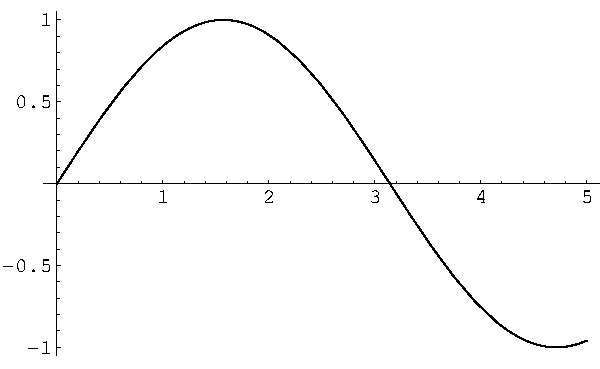
\includegraphics[width=0.4\textwidth]{figs/sin.pdf}}
		%\hfil
		\captionbox{The second subfigure. The second subfigure\label{mini:subb}}[0.49\textwidth]
		{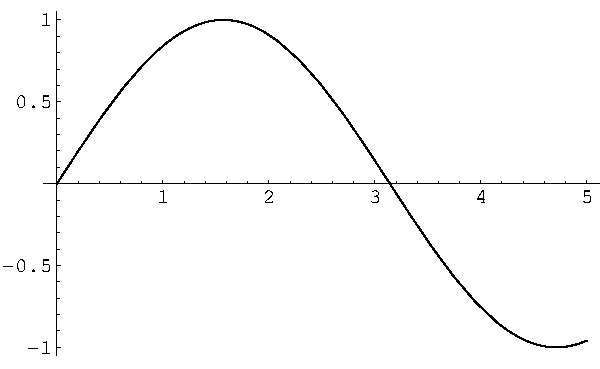
\includegraphics[width=0.4\textwidth]{figs/sin.pdf}}
	\end{figure}

	
	\begin{figure}[htbp] %[H]
		\centering
		\subcaptionbox{The first subfigure. The first subfigure\label{mini:subc}}[0.45\textwidth]
		{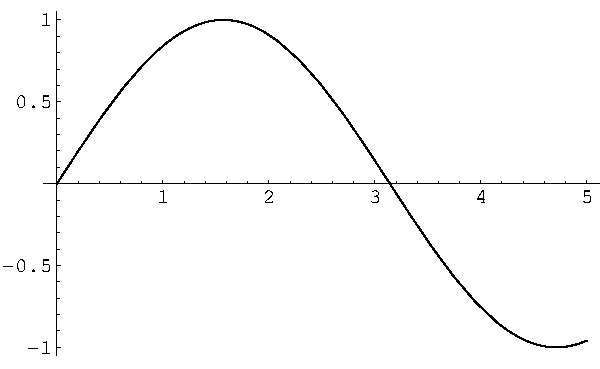
\includegraphics[width=0.4\textwidth]{figs/sin.pdf}}
		%\hfil
		\subcaptionbox{The second subfigure. The second subfigure\label{mini:subd}}[0.45\textwidth]
		{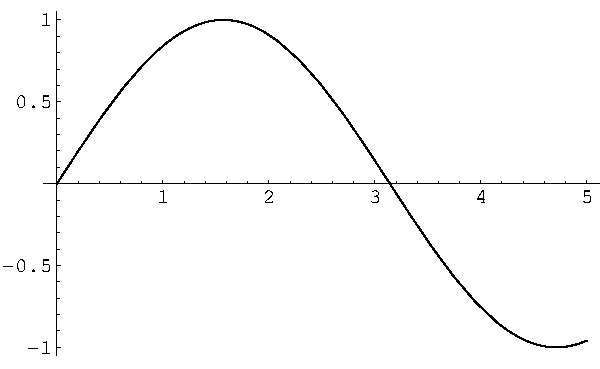
\includegraphics[width=0.4\textwidth]{figs/sin.pdf}}
		\caption{Two subfigures side by side (with subcaptionbox command)}
		\label{mini:subfigs} %% label for entire figure
	\end{figure}
	

	\begin{figure}[H]
		\centering
		\begin{subcaptionblock}{0.45\textwidth}	
			\centering
			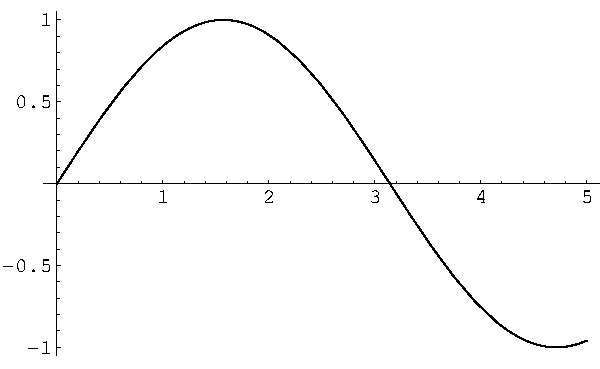
\includegraphics[width=0.8\textwidth]{figs/sin.pdf}
			\caption{The first subfigure.}\label{mini:sube} 
		\end{subcaptionblock}%	
		%\hfil
		\begin{subcaptionblock}{0.45\textwidth}	
			\centering
			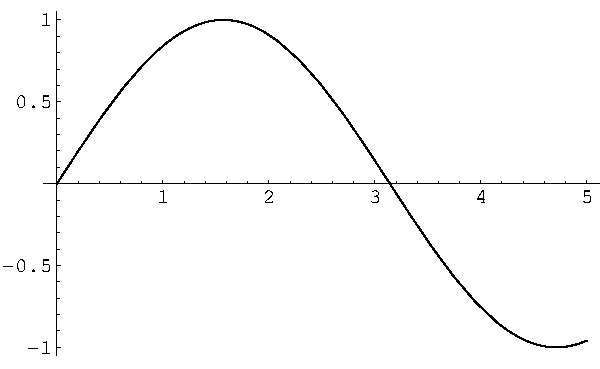
\includegraphics[width=0.8\textwidth]{figs/sin.pdf}
			\caption{The second subfigure.}\label{mini:subf} 
		\end{subcaptionblock}	
		\caption{Two subfigures side by side (with subcaptionblock environment), wrapped in two lines}\label{mini:subfigures} 
	\end{figure}



\subsubsection{Theorems}

\begin{definition} %
This is a definition... .
\end{definition}%
\begin{lemma}%
Here is the content of a lemma.
\end{lemma}
\begin{theorem}\label{thm-1}%
Here is the content of Theorem \ref{thm-1}.
\end{theorem}%
\begin{theorem}\label{thm-2}{\cms[Uniqueness criterion]}\;
	Here is the content of Theorem \ref{thm-2}.
\end{theorem}%
\begin{proof}%
Here comes the proof of Theorem \ref{thm-2}.
\end{proof}
\begin{corollary}%
Here is the content of the corollary.
\end{corollary}
\begin{proposition}
This is a proposition.
\end{proposition}

\subsubsection{Reference fo Floating Objects}
Now comes some examples for formulas, tables and figures being referred to.
\begin{example}
See Equation \eqref{eq:1} on page \pageref{eq:1}.
\end{example}
\begin{example}
See Table \ref{table:1}  on page \pageref{table:1}.
\end{example}
\begin{example}
See Figure \ref{mini:subd} on page \pageref{mini:subd}.
\end{example}
\begin{example}
See Theorem \ref{thm-1} on page \pageref{thm-1}.
\end{example}
		
\subsubsection{Bibiliography and Reference}
	
\begin{example}
Four forms of  in numerical referencing style are defined in this template with the package \texttt{bilatex}, which is used to manage the bibliography. Here are some examples. 
\begin{enumerate}[leftmargin=7.8mm,itemsep=-0.1ex,label= \arabic*)]%\emph{\alph*},(\Roman*),(\arabic*)
\item Usual reference with command \verb|\ncite{}|, e.g.: See \ncite{Shell:2002};
\item Reference with additional information using command \verb|\rcite{}|, e.g.: \rcite{Gai2024}{Page 150}, \rcite{Gai2024}{Section 5};
\item Superscript reference with command \verb|\ucite{}|,e.g.: We can learn \LaTeX{}  further from references \ucite{Voss2014,Gratzer2007,Pakin2024,Goossens2007,Shell:2002}.  		
\item Reference with family name, using command \verb|\ancite{}|, e.g.:  \ancite{Shell:2002}(for one author only), \ancite{zhouxu:2019}(for two authors),  \ancite{Gelman2014}(for at least three authors). 
	\end{enumerate}
\end{example}	

%%%%%%%%%%%%%%%%%%%%%%%%%%%%%%%%%%%%%%%%%%%%%%%%%%%%%%%%%%%%%%%%
%        Appendices                                            %
%%%%%%%%%%%%%%%%%%%%%%%%%%%%%%%%%%%%%%%%%%%%%%%%%%%%%%%%%%%%%%%%
%
\appendix
\numberwithin{equation}{section}
\numberwithin{figure}{section}
\numberwithin{table}{section}
\makeatletter 
% "activate" the preparatory code, but for section-level headers only
\newcommand{\section@cntformat}{Appdendix \thesection:\ }
\makeatother

%%%%%%%%%%%%%%%%%%%%%%%%%%%%%%%%%%%%%%%%%%%%%%%%%%%%%%%%%%%%%%%%
\section{Further Remarks}
%%%%%%%%%%%%%%%%%%%%%%%%%%%%%%%%%%%%%%%%%%%%%%%%%%%%%%%%%%%%%%%%
\begin{remark}
	Equations, tables and figures are numbered separately. See, for example, Equation \eqref{eqn-A1}.
\begin{equation}\label{eqn-A1}
	\widehat{\Theta}=\sum_{z} \frac{n(\boldsymbol{z})}{n}\left\{\widebar{Y}_{a}(\boldsymbol{z})
	-\widetilde{Y}_{b}(\boldsymbol{z})\right\}. 
\end{equation}
	
\end{remark}
\begin{remark}
	See the remarks in the Chinese version.
\end{remark}
\begin{remark}
For futher study on the typesetting based on English-Chinese \LaTeX{} and some special techniques,
please refer to \ncite{Voss2014,Gratzer2007,Pakin2024,Goossens2007,Shell:2002}. 
\end{remark}

\nocite{*}
%\nocite{Shell:2002, Gelman2014,Dalu:1998,focus,zhouxu:2019}

\begin{spacing}{1.0} % 行距
	\printbibliography[keyword={en},resetnumbers=true,
	                   title={\bfseries\sffamily \zihao{-4} References}]
\end{spacing}	

\nolinenumbers

%%%%%%%%%%%%%%%%%%%%%%%%%%%%%%%%%%%%%%%%%%%%%%%%%%%%%%%%%%%%%%%%
%  英文摘要
%%%%%%%%%%%%%%%%%%%%%%%%%%%%%%%%%%%%%%%%%%%%%%%%%%%%%%%%%%%%%%%%
\vspace{6mm}\hspace{-8mm}
\parbox{\textwidth}{
	\begin{center}
        \zihao{-2}{\textbf{\cntitle}}\\[1em]
        \begin{tabular}{c}\zihao{-4}\kaishu\cnfirstauthor\\[-6pt]
	    	\zihao{-5}(\cnfirstinst)\end{tabular}
		\begin{tabular}{c}\zihao{-4}\kaishu\cnsecondauthor\\[-6pt]
			\zihao{-5}(\cnsecondinst)\end{tabular}
	\end{center}
	\textbf{摘~~~要:}\quad{\fangsong\cnabstract}\\
	\textbf{关键词:}\quad{\fangsong\cnkeywords}\\
	\textbf{中图分类号:}\quad\cnclassno}

%
% 作者及单位信息不同格式参考中文论文的模板
% 

%%%%%%%%%%%%%%%%%%%%%%%%%%%%%%%%%%%%%%%%%%%%%%%%%%%%%%%%%%%%%%%%
%  文章结束
%%%%%%%%%%%%%%%%%%%%%%%%%%%%%%%%%%%%%%%%%%%%%%%%%%%%%%%%%%%%%%%%

\clearpage
\end{document}
